% Options for packages loaded elsewhere
\PassOptionsToPackage{unicode}{hyperref}
\PassOptionsToPackage{hyphens}{url}
\PassOptionsToPackage{dvipsnames,svgnames,x11names}{xcolor}
%
\documentclass[]{interact}

\usepackage{epstopdf}% To incorporate .eps illustrations using PDFLaTeX, etc.
\usepackage[caption=false]{subfig}% Support for small, `sub' figures and tables

\usepackage[natbibapa,nodoi]{apacite}% Citation support using apacite.sty. Commands using natbib.sty MUST be deactivated first!
\setlength\bibhang{12pt}% To set the indentation in the list of references using apacite.sty. Commands using natbib.sty MUST be deactivated first!
\renewcommand\bibliographytypesize{\fontsize{10}{12}\selectfont}% To set the list of references in 10 point font using apacite.sty. Commands using natbib.sty MUST be deactivated first!

\let\subcaption\relax
\let\subfloat\relax

\theoremstyle{plain}% Theorem-like structures provided by amsthm.sty
\newtheorem{theorem}{Theorem}[section]
\newtheorem{lemma}[theorem]{Lemma}
\newtheorem{corollary}[theorem]{Corollary}
\newtheorem{proposition}[theorem]{Proposition}

\theoremstyle{definition}
\newtheorem{definition}[theorem]{Definition}
\newtheorem{example}[theorem]{Example}

\theoremstyle{remark}
\newtheorem{remark}{Remark}
\newtheorem{notation}{Notation}

\usepackage{amsmath,amssymb}
\usepackage{iftex}
\ifPDFTeX
  \usepackage[T1]{fontenc}
  \usepackage[utf8]{inputenc}
  \usepackage{textcomp} % provide euro and other symbols
\else % if luatex or xetex
  \usepackage{unicode-math}
  \defaultfontfeatures{Scale=MatchLowercase}
  \defaultfontfeatures[\rmfamily]{Ligatures=TeX,Scale=1}
\fi
\usepackage{lmodern}
\ifPDFTeX\else  
    % xetex/luatex font selection
\fi
% Use upquote if available, for straight quotes in verbatim environments
\IfFileExists{upquote.sty}{\usepackage{upquote}}{}
\IfFileExists{microtype.sty}{% use microtype if available
  \usepackage[]{microtype}
  \UseMicrotypeSet[protrusion]{basicmath} % disable protrusion for tt fonts
}{}
\makeatletter
\@ifundefined{KOMAClassName}{% if non-KOMA class
  \IfFileExists{parskip.sty}{%
    \usepackage{parskip}
  }{% else
    \setlength{\parindent}{0pt}
    \setlength{\parskip}{6pt plus 2pt minus 1pt}}
}{% if KOMA class
  \KOMAoptions{parskip=half}}
\makeatother
\usepackage{xcolor}
\setlength{\emergencystretch}{3em} % prevent overfull lines
\setcounter{secnumdepth}{5}
% Make \paragraph and \subparagraph free-standing
\ifx\paragraph\undefined\else
  \let\oldparagraph\paragraph
  \renewcommand{\paragraph}[1]{\oldparagraph{#1}\mbox{}}
\fi
\ifx\subparagraph\undefined\else
  \let\oldsubparagraph\subparagraph
  \renewcommand{\subparagraph}[1]{\oldsubparagraph{#1}\mbox{}}
\fi


\providecommand{\tightlist}{%
  \setlength{\itemsep}{0pt}\setlength{\parskip}{0pt}}\usepackage{longtable,booktabs,array}
\usepackage{calc} % for calculating minipage widths
% Correct order of tables after \paragraph or \subparagraph
\usepackage{etoolbox}
\makeatletter
\patchcmd\longtable{\par}{\if@noskipsec\mbox{}\fi\par}{}{}
\makeatother
% Allow footnotes in longtable head/foot
\IfFileExists{footnotehyper.sty}{\usepackage{footnotehyper}}{\usepackage{footnote}}
\makesavenoteenv{longtable}
\usepackage{graphicx}
\makeatletter
\def\maxwidth{\ifdim\Gin@nat@width>\linewidth\linewidth\else\Gin@nat@width\fi}
\def\maxheight{\ifdim\Gin@nat@height>\textheight\textheight\else\Gin@nat@height\fi}
\makeatother
% Scale images if necessary, so that they will not overflow the page
% margins by default, and it is still possible to overwrite the defaults
% using explicit options in \includegraphics[width, height, ...]{}
\setkeys{Gin}{width=\maxwidth,height=\maxheight,keepaspectratio}
% Set default figure placement to htbp
\makeatletter
\def\fps@figure{htbp}
\makeatother
\newlength{\cslhangindent}
\setlength{\cslhangindent}{1.5em}
\newlength{\csllabelwidth}
\setlength{\csllabelwidth}{3em}
\newlength{\cslentryspacingunit} % times entry-spacing
\setlength{\cslentryspacingunit}{\parskip}
\newenvironment{CSLReferences}[2] % #1 hanging-ident, #2 entry spacing
 {% don't indent paragraphs
  \setlength{\parindent}{0pt}
  % turn on hanging indent if param 1 is 1
  \ifodd #1
  \let\oldpar\par
  \def\par{\hangindent=\cslhangindent\oldpar}
  \fi
  % set entry spacing
  \setlength{\parskip}{#2\cslentryspacingunit}
 }%
 {}
\usepackage{calc}
\newcommand{\CSLBlock}[1]{#1\hfill\break}
\newcommand{\CSLLeftMargin}[1]{\parbox[t]{\csllabelwidth}{#1}}
\newcommand{\CSLRightInline}[1]{\parbox[t]{\linewidth - \csllabelwidth}{#1}\break}
\newcommand{\CSLIndent}[1]{\hspace{\cslhangindent}#1}

\usepackage{booktabs}
\usepackage{longtable}
\usepackage{array}
\usepackage{multirow}
\usepackage{wrapfig}
\usepackage{float}
\usepackage{colortbl}
\usepackage{pdflscape}
\usepackage{tabu}
\usepackage{threeparttable}
\usepackage{threeparttablex}
\usepackage[normalem]{ulem}
\usepackage{makecell}
\usepackage{xcolor}
\usepackage{siunitx}

  \newcolumntype{d}{S[
    input-open-uncertainty=,
    input-close-uncertainty=,
    parse-numbers = false,
    table-align-text-pre=false,
    table-align-text-post=false
  ]}
  
\makeatletter
\makeatother
\makeatletter
\makeatother
\makeatletter
\@ifpackageloaded{caption}{}{\usepackage{caption}}
\AtBeginDocument{%
\ifdefined\contentsname
  \renewcommand*\contentsname{Table of contents}
\else
  \newcommand\contentsname{Table of contents}
\fi
\ifdefined\listfigurename
  \renewcommand*\listfigurename{List of Figures}
\else
  \newcommand\listfigurename{List of Figures}
\fi
\ifdefined\listtablename
  \renewcommand*\listtablename{List of Tables}
\else
  \newcommand\listtablename{List of Tables}
\fi
\ifdefined\figurename
  \renewcommand*\figurename{Figure}
\else
  \newcommand\figurename{Figure}
\fi
\ifdefined\tablename
  \renewcommand*\tablename{Table}
\else
  \newcommand\tablename{Table}
\fi
}
\@ifpackageloaded{float}{}{\usepackage{float}}
\floatstyle{ruled}
\@ifundefined{c@chapter}{\newfloat{codelisting}{h}{lop}}{\newfloat{codelisting}{h}{lop}[chapter]}
\floatname{codelisting}{Listing}
\newcommand*\listoflistings{\listof{codelisting}{List of Listings}}
\makeatother
\makeatletter
\@ifpackageloaded{caption}{}{\usepackage{caption}}
\@ifpackageloaded{subcaption}{}{\usepackage{subcaption}}
\makeatother
\makeatletter
\@ifpackageloaded{tcolorbox}{}{\usepackage[skins,breakable]{tcolorbox}}
\makeatother
\makeatletter
\@ifundefined{shadecolor}{\definecolor{shadecolor}{rgb}{.97, .97, .97}}
\makeatother
\makeatletter
\makeatother
\makeatletter
\makeatother
\ifLuaTeX
  \usepackage{selnolig}  % disable illegal ligatures
\fi
\IfFileExists{bookmark.sty}{\usepackage{bookmark}}{\usepackage{hyperref}}
\IfFileExists{xurl.sty}{\usepackage{xurl}}{} % add URL line breaks if available
\urlstyle{same} % disable monospaced font for URLs
\hypersetup{
  pdftitle={Lonely and online: an investigation of social media use and social isolation in China},
  pdfkeywords={Social Isolation, Social Media, Digital
Communication, China},
  colorlinks=true,
  linkcolor={blue},
  filecolor={Maroon},
  citecolor={Blue},
  urlcolor={Blue},
  pdfcreator={LaTeX via pandoc}}


\begin{document}
\title{Lonely and online: an investigation of social media use and
social isolation in China}



\author{\name{\textsuperscript{a} and }
\affil{\textsuperscript{a}
\textsuperscript{b}}}

\maketitle

\begin{abstract}
Research on the link between social media and well being has lead to
ambiguous findings - some research has found a positive, negative, and
mixed relationship between the two. We employ the case of China, in
which social media is controlled in important ways, as a useful
alternative case to gain leverage on these ambiguities. Using data from
a nationwide survey of Chinese citizens (n=2292), we principally find
that individual, heterogeneous effects are an important driver of the
relationship between levels of social media use and reported well-being.
Additionally, our results lend support to a FOMO (fear of missing out)
mechanism as an important driver of the relationship while not finding
support for the mechanism of exposure to negative content on social
media as a predictor of well-being. Finally, our findings suggest that
institutional context may not play an important role in the social media
- social isolation relationship.
\end{abstract}

\begin{keywords}
    Social Isolation, Social Media, Digital Communication, 
    China
\end{keywords}\ifdefined\Shaded\renewenvironment{Shaded}{\begin{tcolorbox}[breakable, frame hidden, enhanced, borderline west={3pt}{0pt}{shadecolor}, sharp corners, boxrule=0pt, interior hidden]}{\end{tcolorbox}}\fi

\newpage{}

\hypertarget{introduction}{%
\section{Introduction}\label{introduction}}

Research is quite mixed when it comes to identifying the relationship
between social media use and feelings of isolationism. Early research
suggested that the internet would build social capital, or an
interconnectedness between people, and that social media platforms were
the ultimate way to bring people together (Ellison et al., 2007). Since
then, research on the subject has been decidedly more mixed (Duradoni et
al., 2020; Jiménez et al., 2022; Valkenburg et al., 2022). On one hand,
some authors have found social media may encourage social isolation, and
ultimately, social media users may feel more disconnected from others
than those who do not use social media. On the other hand, others have
found that there is only a minimal relationship between these two
variables. More recent scholarship has suggested that social media use
may produce heterogeneous effects on individuals' sense of well-being
(Ivie et al., 2020; Ostic et al., 2021).

This study uses the little-studied Chinese social media environment to
answer two research questions that remain unresolved in the literature:
1) through which channels or mechanisms do possible heterogeneous
effects operate through and 2) how much does internet context change the
relationship between social isolation and social media use. The reason
that we believe the case of China can be helpful in answering these
question is that Chinese online environment has certain features that
should both moderate and exacerbate key causal pathways previously
identified in the literature. To resolve these debates, we employ a
large survey (n=2292) of Chinese internet users and test a variety of
regression specifications.\footnote{All data and analysis files for this
  research are available at the author's website.} The main result is
that social media use is generally negatively related to social
isolation, though the nature of this relationship changes depending on
the urbanicity of the respondent - being in a rural area amplifies this
relationship. These results are consistent with a mechanism that links
the two via the harmfulness of being exposed to constant online
comparisons (so-called FOMO or fear of missing out). However, the
contextual differences of the Chinese internet compared to the Western
internet do not appear to significantly alter the relationship.

\hypertarget{literature-review-and-theory}{%
\section{Literature Review and
Theory}\label{literature-review-and-theory}}

Initially, scholars imagined that social media would create more
opportunities for users to create unique and fulfilling social
relationships (Ellison et al., 2007; Steinfield et al., 2008;
Subrahmanyam et al., 2008). The early theorizing about the possible
benefits of social media hypothesized three important mechanisms by
which social media could decrease loneliness. 1) creating more
opportunities for online to offline meetups and 2) helping to alleviate
feelings of isolation for those who have difficulty making in-person
social connections via joining an online communities, and 3)
facilitating keeping in touch with family and friends.

More recent studies on the subject have found significantly more mixed
and often negative evidence regarding the impact of social media on
feelings of isolation. Primack et al.~found a negative relationship
between social media use and social isolation in youth in a
representative sample (Primack et al., 2017). A meta-review of the
literature on adolescent social media usage notes that while the effect
size is often small the relationship in most studies on social media's
linkage to ill-being is negative (Valkenburg et al., 2022) while
emphasizing the importance of heterogeneous effects. There are
relatively fewer studies that consider all ages. However, those that
have been conducted also emphasize that the relationship between social
media use and well-being has possible negative effects but the effects
seem to vary by personality type (Appel et al., 2020). More recent
research has reinforced the finding that the effect of social media on
measures like social isolation may be highly heterogeneous across
individuals; for some individuals, the effect may be quite negative for
some while for others social media usage may have a modestly positive
impact on well-being (Beyens et al., 2020; Ostic et al., 2021). For
example, for some users moderate social media use may have no
significant impact but for those who suffer from social media addiction,
the effect can be highly negative (Alhassan et al., 2018; Aljomaa et
al., 2016) (though see (Al-Kandari \& Al-Sejari, 2021; Chen et al.,
2017) for more complex findings).

While most of the studies agree that the causal direction flows from
social media use to feelings of isolation (though see (Kim, 2017;
Nowland et al., 2018)), there is disagreement among authors about the
specific mechanisms and causal pathways through which this relationship
exists. For those who find a negative relationship between social media
and well-being, one set of mechanisms suggests that the social media
itself that is the problem. Cyberbullying, or more generally, repeated
and aggressive online attacks against users has been systematically
linked to feelings of social isolation (Ademiluyi et al., 2022). Another
proposed mechanism is upward comparisons of others - users observe
content of friends or influencers who post luxurious or exotic
experiences which cause users to encounter feelings of unhappiness or
FOMO about their own life situation (Alabri, 2022; Büttner \& Rudert,
2022). A third set of mechanisms primarily concern themselves with the
physical changes that social media causes. Social media use has been
shown to displace face to face activity, which leads to greater social
isolation (Larson et al., 2018). The current research suggests that
which of these mechanisms is dominant depends on the age/demographic
group in question and the societal context (Twenge, 2019).

Most of the existing research on the subject focuses on Western highly
developed societies, and this focus limits variation on key independent
variables given the similar social and institutional context in which
users are embedded. To address this problem, this study aims to
understand how these complex dynamics interact in the non-Western
setting of China. We believe the setting of China gives additional
leverage to investigate issues of heterogeneity and the importance of
context for several reasons. Firstly, the highly controlled nature of
China's internet space prevents user exposure to some of the more
threatening online content (such as cyberbullying) that is hypothesized
to be a factor in creating a negative relationship between social media
and feelings of social isolation (Wang, 2020). If this mechanism were
the dominant reason for previous findings of a negative relationship
between the two, one would expect the relationship to be more positive
in China. Relatedly, China has a more commercial and robust influencer
culture that often dominates user's social media consumption (Tam, 2019;
Wei, 2023). If the main pathway creating a negative relationship is via
user's comparisons of their lives with others (FOMO), we expect the
relationship between social media use and feelings of social isolation
to be greater in China.

Finally, China has undergone a period of very rapid urbanization in the
last 40 years, a development that has brought about enormous changes to
traditional social structures (Xu \& Xia, 2014). This rapid urbanization
can help test two important unresolved questions in the existing
literature that are difficult to resolve given that urbanization in
Western countries is a process that largely finished by the advent of
social media. The first is whether social media can provide a means to
decrease social isolation among those who actively seek it out to make
friends. China's rapid urbanization and attendant human migration has
created a large population of people that lack strong social bonds and
may use social media as a method to create new social bonds (as the
earlier theorists of social media hypothesized users may employ the
technology). The existing literature on the West finds that urbanicity
is an important factor in levels and mechanisms for social isolation;
many studies of Western societies have found that rural residents, while
having stronger familial bonds, also can more easily experience social
isolation without those bonds (Henning-Smith et al., 2018; Kaye, 2017;
Koning et al., 2017). Social media use in China could therefore either
help mitigate the feelings of isolation brought on by rapid urbanization
by connecting family members who have left the countryside for urban
work (based on the earlier, more positive views of social media's
potential) or amplify further the feelings of isolation due to several
of the proposed negative relationship mechanisms.

The case of China cannot resolve every debate in the literature or test
all possible mechanisms but we do believe it can provide insight into a
few of the more prominent proposed processes. Thus, given the existing
literature and the context of China, we develop a series of testable
hypotheses that shed light on our research question.

\begin{itemize}
\item
  \textbf{H\(1_a\)}: social media use should have a positive connection
  to social isolation due to strengthened government control over online
  content
\item
  \textbf{H\(1_b\)}: social media use should have a negative connection
  to social isolation due to the dominance of influencer culture in
  China, moderated by age.
\item
  \textbf{H\(2\)}: those who are able to use social media to make new
  friends will have lower social isolation scores than those who do not
\item
  \textbf{H\(3\):} the urban/rural divide will produce differential
  impacts in the above hypotheses on the relationship between social
  media use and social isolation
\end{itemize}

\hypertarget{data-measurement-and-descriptives}{%
\section{Data, Measurement, and
Descriptives}\label{data-measurement-and-descriptives}}

The data used in this study are original. We designed a survey
instrument in English, and translated it into Chinese, to measure a
range of concepts including social isolationism and various dimensions
of social media and digital information consumption. We employed
Qualtrics to collect the data. They randomly selected 2292 respondents
from their existing panel\footnote{Qualtrics recruits a large pool of
  respondents for various survey projects through online advertising.
  Recruits who update their profiles at least once every 6 months are
  randomly invited to participate. These recruits are awarded online
  points that can be exchanged for cash or various other
  country-specific gifts. The number of points is based on the length of
  the survey, and since our survey had over fifty questions, respondents
  received a relatively high number of points.} from November 25 to
December 2, 2015. This sample size on provides for a roughly \(\pm2\)
margin of error.\footnote{We were able to first collect a small sample
  (\(n=286\)) to check the reliability and adjust the instrument after
  before proceeding with the final data collection. We made three
  adjustments, none of which are related to the measures used in the
  current study.} While our sample is selected randomly from Qualtrics'
online user panel, it isn't representative of China's entire population
due to its internet-based recruitment methods. The sample, however,
aligns well with Chinese internet users, crucial for our internet
effects research. Compared to national data, our sample skews younger
and more educated but is similar in income and gender.\footnote{See
  https://data.worldbank.org/country/china (go to the Country Profile),
  and
  https://www.cnnic.com.cn/AU/Introduction/Introduction/201208/t20120815\_33295.htm.}
These demographics reflect the global digital divide and are in line
with expectations for internet users in developing regions. Our findings
are particularly relevant for understanding digital media's impact among
active internet users in China.

Our dependent variable, \emph{social isolationism}, is a three-item
additive index. Respondents were given the following introduction: The
next question is about how you feel about different aspects of your
life. Could you tell me for each one if you feel that way always, almost
always, some of the time, rarely or never? Then they were asked: A) How
often do you feel that you lack companionship, B) How often do you feel
isolated from others?, and C) How often do you feel left out? Response
options were recoded so that higher responses equated to feeling more
socially isolated, they were all three added together, and then rescaled
to range from 0 through 1 maintaining the original intervals
(\(\alpha = 0.86\)). The distribution of that index is presented in
Figure~\ref{fig-social-iso-dist}. The distribution is relatively normal
centered around the midpoint with a slight skew to the right. Most
respondents appear to be on the low end, indicating the the majority of
those in our sample do not feel particularly isolated. Conversely, the
right skew in the distribution does suggest that a sizable chunk of
folks feel quite socially isolated. Altogether, the spread out
distribution indicates quite a bit of variance (\(\mu = 0.41\),
\(sd = 0.20\)).

\begin{figure}

{\centering 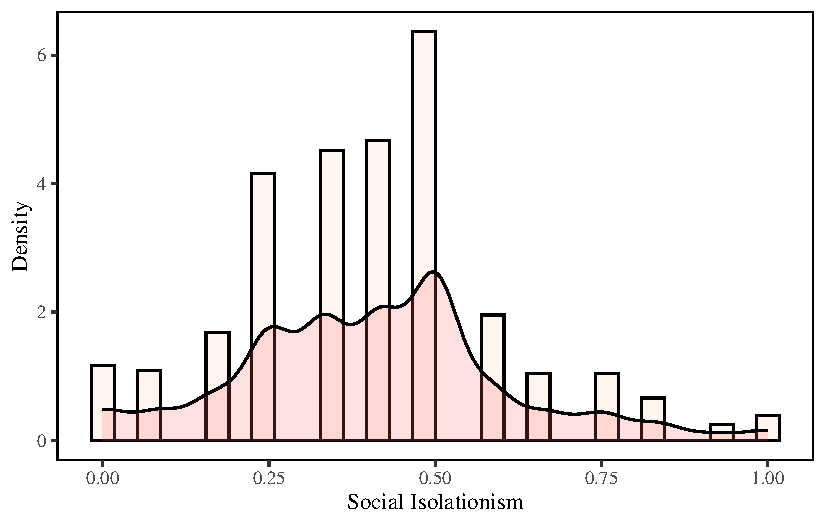
\includegraphics{Social-Isolation-in-China-jg-revised_files/figure-pdf/fig-social-iso-dist-1.pdf}

}

\caption{\label{fig-social-iso-dist}Distribution of Social Isolationism
Index}

\end{figure}

We have several primary independent variables including human
interaction, online to offline relationships, general social media use,
and urbanicity. We measured human interaction with a single item: ``Has
the internet and phone applications increased your contact with the
following groups of people (check yes to all that apply)?'' The response
options were: 1) Family that lives nearby, 2) Family that lives far
away, 3) Friends that live nearby, 4) Friends that live far away, 5)
People you met on the internet that live nearby, and 6) People you met
on the internet that live far away. We simply counted the number of
selected responses so the item ranged from 0 to 6, and then for the
models that come later, we rescaled it to range from 0 through 1
maintaining the original intervals. Online to offline relationships was
also measured with a single item: Have you met someone offline that you
initially met online? Response options were: 1) Yes, many times, 2) Yes,
several times, 3) Yes, once, and 4) No, never. We inverted this scale so
that higher values represented more offline relationships, and again,
rescaled it to range from 0 through 1 for the models that follow.

The distributions of these ordinal independent variables are reflected
in Figure~\ref{fig-var-dist}. Very few people claimed to never have
increased their contact/connections with others through the internet.
The modal number of increased connections respondents claimed to have
made through the internet was 2, followed closely by 1, but a sizable
proportion of the sample, about 48\% claimed to have increased their
number of personal connections by 3 or more through the internet.
Perhaps not surprisingly, the modal response when asked whether one had
met someone online and that relationship moved offline was ``No,
never''. On the other hand, we were surprised that about 37\% of those
sampled claimed to have moved relationships offline several times, over
10\% said they had done so many times, and about 13\% did so once. Taken
altogether, a large proportion of our respondents seem to using the
internet to facilitate social relations.

\begin{figure}

{\centering 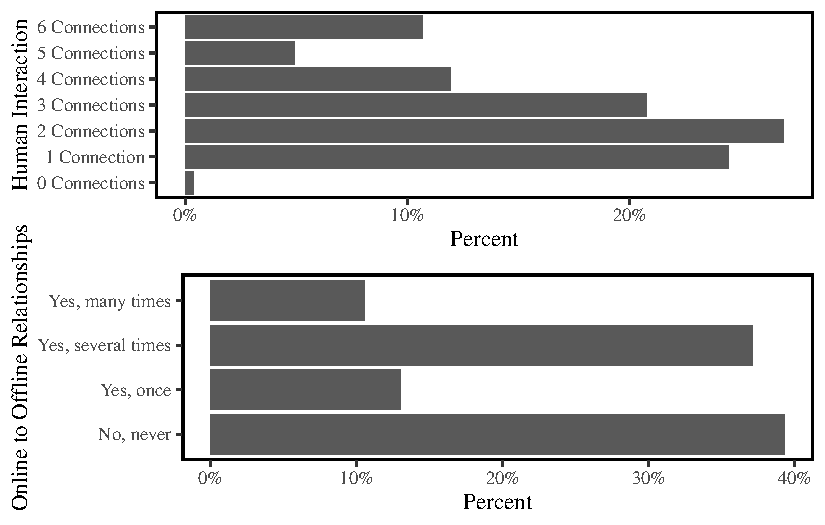
\includegraphics{Social-Isolation-in-China-jg-revised_files/figure-pdf/fig-var-dist-1.pdf}

}

\caption{\label{fig-var-dist}Primary Independent Variables
Distributions}

\end{figure}

We measured general social media use with an index based on the
following three items: 1) About how many hours a day would you estimate
you spend using only social media? Social media means applications like
Weibo, QQ, Renren, Kaixin001, Douban, WeChat or other sites and services
that allow users to interact with each other. (0-1, 1-2, 2-3, 3-4, 4-5,
5-6, 6-7, 7-8, 8-9, or More than 9), 2) Do you check email, read
websites, and use social media (social media means applications like
Weibo, QQ, Renren, Kaixin001, Douban, WeChat or other sites and services
that allow users to interact with each other) more than you did five
years ago? (Yes, No), and 3) How often do you read news stories about
political events that have been posted on social media (social media
means applications like Weibo, QQ, Renren, Kaixin001, Douban, WeChat or
other sites and services that allow users to interact with each other)?
(More than once a day, Everyday, Three-to-five days per week, One-to-two
days per week, Less often, Never). Each was recoded so that higher
values represented more social media use, rescaled to range from 0
through 1, added together, and then again, rescaled to range from 0
through 1 maintaining all original intervals.The Chronbach's alpha was
relatively low for these three items (\(\alpha = 0.31\)), but we
proceeded with the construction of this index because, first, the face
validity is high. Simply, those who claim to use social media generally
more often, claim to read political news more often, and claim to use it
more than they did in the past, are certainly likely to be more frequent
social media users than those who do not do all these things.Second, we
confirmed that these three items were all positively correlated with
each other (p \textless{} 0.0001 for all pairwise relationships). The
distribution of this index is presented in Figure~\ref{fig-sm-use-dist}.
The distribution is relatively normal and tightly centered around the
mean 0.63 with a standard deviation of 0.17, but there is a left skew
suggesting that a portion of the population is not that social media
active, but clearly the bulk of the population are.

\begin{figure}

{\centering 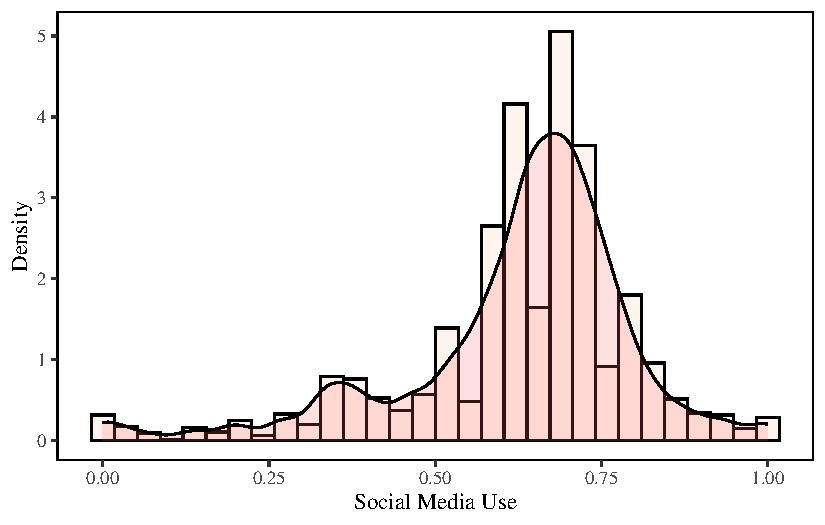
\includegraphics{Social-Isolation-in-China-jg-revised_files/figure-pdf/fig-sm-use-dist-1.pdf}

}

\caption{\label{fig-sm-use-dist}General Social Media Use Distribution}

\end{figure}

Our final primary independent variable, urbanicity, was measured using a
single item: Which of these best describes the place in which you live?
(Countryside/Village, Small City, Mid-Sized City, Suburban Area of a Big
City, Big City). For the purpose of the models, we rescaled this item to
range from 0 through 1 maintaining the original intervals. The
distribution is reflected in Figure~\ref{fig-urban-dist}. Given the
rural to urban Chinese migration since the founding of the People's
Republic (Xia, 1995), it is not surprising to see that nearly 45\% of
those in our sample live in cities, 7\% in suburbs, and about 27\% in
mid-sized cities. About 16\% say they live in small cities and only
about 5\% say they live in villages.

\begin{figure}

{\centering 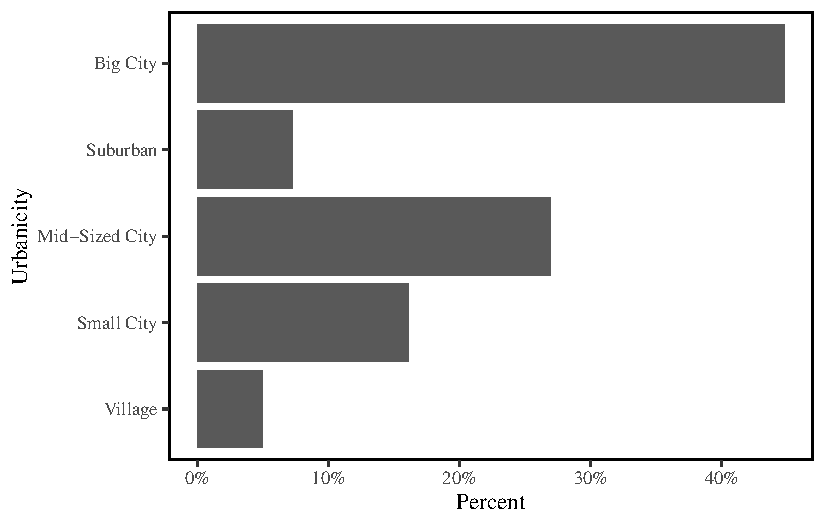
\includegraphics{Social-Isolation-in-China-jg-revised_files/figure-pdf/fig-urban-dist-1.pdf}

}

\caption{\label{fig-urban-dist}Urbanicity Distribution}

\end{figure}

Our modeling strategy that follows is straightforward. We begin by
modeling each of our internet communication independent variables as
function of socio-economic status (SES), gender, Chinese Communist Party
membership (CCP), and age to create an individual profile of each type
of digital user (see the Online Appendix for the operationalization of
these variables). This provides some context for the models that follow
which are intended to test our primary hypotheses, that is that internet
communication can deter social isolation and that this is particularly
true for those who do not have the convenience of the high social
interaction opportunity provided by urban living. For those we begin by
fitting an additive model of our index of social isolationism as
function of each of our primary independent variables while also
controlling for the same variables included in our profile models.
Finally, we refit three models with the same specification but introduce
an interactive term between each of our internet communication
indicators, respectively, with our measure of urbanicity. This allows us
to test whether the observed additive effects are stronger for those
living outside cities.

\hypertarget{results}{%
\section{Results}\label{results}}

Given that the first two dependent variables (human interaction, online
to offline to offline relationships) in our profile models are
distributed ordinally, we initially estimate linear models of those
outcomes and examine the residual behavior to determine if a linear
model fits the data well or if an ordered outcome model is a better fit.
The results were clear, a linear model is not a good fit for either
outcome (see the figures in the Online Appendix), so we fit the models
using ordered logit. Because our measure of general social media is
based on an additive index, we treat it as continuous, and accordingly
fit a linear model.

\hypertarget{tbl-profile-models}{}
\begin{table}
\caption{\label{tbl-profile-models}Modeling Profiles of Digital Communication }\tabularnewline

\centering
\begin{threeparttable}
\begin{tabular}[t]{lccc}
\toprule
  & Human Interaction & Online/Offline Interaction & General Social Media\\
\midrule
SES & \num{2.35}* & \num{2.16}* & \num{0.24}*\\
 & (\num{0.27}) & (\num{0.28}) & (\num{0.03})\\
Female & \num{-0.03} & \num{-0.35}* & \num{0.01}\\
 & (\num{0.08}) & (\num{0.08}) & (\num{0.01})\\
CCP Member & \num{-0.17} & \num{0.23}* & \num{0.01}\\
 & (\num{0.09}) & (\num{0.09}) & (\num{0.01})\\
Age & \num{0.51}* & \num{-0.82}* & \num{-0.12}*\\
 & (\num{0.26}) & (\num{0.27}) & (\num{0.02})\\
\midrule
N & \num{2277} & \num{2276} & \num{2198}\\
Pseudo R2 & \num{0.07} & \num{0.05} & \\
R2 &  &  & \num{0.05}\\
\bottomrule
\multicolumn{4}{l}{\rule{0pt}{1em}* p $<$ 0.05}\\
\end{tabular}
\begin{tablenotes}
\item \textit{Note: } 
\item Human Interaction and Offline/Online Relationships estimates are derived from ordered logit and General Social Media from ordinary least squares.
\end{tablenotes}
\end{threeparttable}
\end{table}

The results of our profile models are presented in
Table~\ref{tbl-profile-models}. When it comes to SES, the relationship
across all three of our internet communication is consistent. As SES
goes up so does digital human interaction, the move from online to
offline relationships, and general social media use. That gender is only
statistically significant in the model of the move from online to
offline relationships where women are less likely to do so.
Interestingly, being a CCP member has inverse relationships with human
interaction and the move from online to offline, where members are less
likely to increase digital human interaction but are more likely to move
online relationships offline. Finally, the older respondents were the
more likely they were to increase human interaction, and the less likely
they were to move relationships offline and use social media. These
profile results provide background context for the models that follow.
The internet communication indicators are our primary independent
variables, so these profile models give us a sense for whom they matter
the most when it comes to deterring social isolation.

\hypertarget{tbl-social-isolation-models}{}
\begin{table}
\caption{\label{tbl-social-isolation-models}Modeling Social Isolation }\tabularnewline

\centering
\begin{threeparttable}
\begin{tabular}[t]{lcccc}
\toprule
  & (1) & (2) & (3) & (4)\\
\midrule
Human Interaction & \num{-0.14}* & \num{-0.04} & \num{-0.14}* & \num{-0.14}*\\
 & (\num{0.02}) & (\num{0.04}) & (\num{0.02}) & (\num{0.02})\\
Online-Offline & \num{0.07}* & \num{0.07}* & \num{0.15}* & \num{0.07}*\\
 & (\num{0.01}) & (\num{0.01}) & (\num{0.03}) & (\num{0.01})\\
Social Media & \num{0.05}* & \num{0.05}* & \num{0.05}* & \num{0.13}*\\
 & (\num{0.03}) & (\num{0.02}) & (\num{0.02}) & (\num{0.05})\\
Urbanicity & \num{-0.04}* & \num{0.02} & \num{0.01} & \num{0.04}\\
 & (\num{0.01}) & (\num{0.03}) & (\num{0.02}) & (\num{0.05})\\
SES & \num{-0.04} & \num{-0.04} & \num{-0.04} & \num{-0.04}\\
 & (\num{0.03}) & (\num{0.03}) & (\num{0.03}) & \vphantom{1} (\num{0.03})\\
Female & \num{0.02}* & \num{0.02}* & \num{0.02}* & \num{0.02}*\\
 & (\num{0.01}) & (\num{0.01}) & (\num{0.01}) & \vphantom{1} (\num{0.01})\\
CCP Member & \num{0.00} & \num{0.00} & \num{0.00} & \num{0.00}\\
 & (\num{0.01}) & (\num{0.01}) & (\num{0.01}) & (\num{0.01})\\
Age & \num{-0.19}* & \num{-0.20}* & \num{-0.20}* & \num{-0.20}*\\
 & (\num{0.03}) & (\num{0.03}) & (\num{0.03}) & (\num{0.03})\\
Human Interaction*Urbanicity &  & \num{-0.14}* &  & \\
 &  & (\num{0.05}) &  & \\
Online-Offline*Urbanicity &  &  & \num{-0.12}* & \\
 &  &  & (\num{0.03}) & \\
Social Media*Urbanicity &  &  &  & \num{-0.13}\\
 &  &  &  & (\num{0.07})\\
\midrule
N & \num{2173} & \num{2173} & \num{2173} & \num{2173}\\
R2 & \num{0.08} & \num{0.08} & \num{0.09} & \num{0.08}\\
\bottomrule
\multicolumn{5}{l}{\rule{0pt}{1em}* p $<$ 0.05}\\
\end{tabular}
\begin{tablenotes}
\item \textit{Note: } 
\item Estimates are derived using ordinary least squares
\end{tablenotes}
\end{threeparttable}
\end{table}

The results of our models of social isolation are presented in
Table~\ref{tbl-social-isolation-models}. The additive estimates in model
(1) provide mixed results regarding whether internet communication is a
positive force in deterring social isolation. Not surprisingly, there is
a negative relationship between the number of digital connections (human
interaction) folks make and feelings of social isolation. On the other
hand, though, both moving online relationships offline and general
social media use are positively related to feelings of social isolation.
The latter is consistent with much of the literature outlined above, but
the former is not. The results also indicate that those living in more
urban environments tend to feel less socially isolated.

Models (2) - (4) in Table 2 include each of the interactions between our
three internet communication measures and urbanicity. The consistent
result across the interactions is that the relationships are dulled for
those living in more rural areas. The interaction between digital humna
interaction and urbanicity is statistically significant (\(p < 0.01\)),
as is that between the move from online to offline relationships and
urbanicity (\(p < 0.001\)), and that between general social media use
and urbanicity only slightly misses the arbitrary \(0.05\) threshold
(\(p = 0.07\)). The interactions are most easily interpreted graphically
(see Figure~\ref{fig-social-isolation-interactions}).

\begin{figure}

{\centering 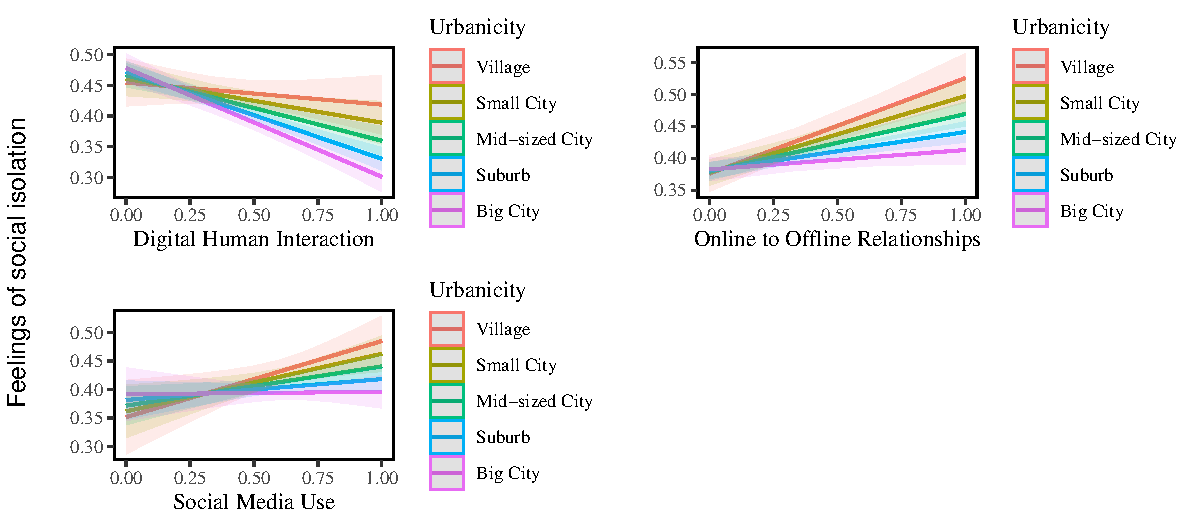
\includegraphics{Social-Isolation-in-China-jg-revised_files/figure-pdf/fig-social-isolation-interactions-1.pdf}

}

\caption{\label{fig-social-isolation-interactions}Modeling Social
Isolation: Interaction Results}

\end{figure}

The model (2) results are graphed in the upper left hand figure. Here it
is clear that the negative relationship between digital human
interaction and feelings of social isolation is considerably stronger
for those in cities. For that matter, notice that the relationship for
those in villages is basically flat; the 95 percent confidence interval
around the slight negative slope indicates that the relationship could
be flat.

The results from the interaction between online to offline relationships
and urbanicity are displayed in the graph in the upper right hand corner
of Figure 5. Again, here, the main effects run in the opposite direction
than those of digital human interaction. Those who are more likely to
move relationships from online to offline tend to feel more isolated,
and the interactive results presented here suggest that this relations
is stronger for those living in less urban spaces. Likewise, the same is
the case for those using social media more frequently. In fact, the
relationship here for those living in the largest cities is completely
non-existent.

In terms of our original hypotheses, we find support for the idea that
China's social media environment is not particularly unique with respect
to generating feelings of social isolation (\textbf{H1b}). Whether or
not this is due to the influencer culture or other factors, we cannot
say with our data, however age is a consistently negative predictor of
social isolation even when controlling for amount of social media use.
This result is at least suggestive of the negative online influencer
culture. We also find, as has been found in other studies, that users
who use the internet to create new connections are less likely to feel
isolated (\textbf{H2}). However, this does not seem to extend to those
that use the internet to facilitate offline meetups. Finally, we find
that the impact of the internet and social media vary significantly
according to the level of urbanicity (\textbf{H3}) - this matches with
previous findings that suggest that there is significant heterogeneity
in the impact of social media on social isloation.

\hypertarget{conclusion}{%
\section{Conclusion}\label{conclusion}}

Cyberoptimists heralded the internet as means by which people could
connect, build social capital, and some suggested this could deter
social isolationism. On the other hand, more recent research and popular
media coverage of the subject has presented a deeply negative view of
the role of social media. Our results do lean toward supporting the
negative conclusions but add important contextualization and are
suggestive of which of the hypothesized mechanisms are most relevant.

Firstly, we found no evidence that the internet could serve as bridge to
build connections for those living outside of cities. The optimistic
view that internet use could lower the costs of making connections for
those who have less social opportunity, those living in less populated
areas, and as a result, help them to feel less isolated. We, in fact,
found the opposite. Internet communication had either less positive
effect or more negative effect on feelings of social isolation for those
living in less urban spaces. This finding lends support to the FOMO
channel - viewing lots of content from influencers in a rural area
compounds feelings of isolation.

Additionally, given the robustly negative relationship between social
media use and social isolation even in the context of China's highly
policed internet, our results cast some doubt on theories that suggest
it is the negative content, such as cyberbullying or violent/graphic
posts, that drives the relationship. Finally, our results also further
suggest more work needs to be done in identifying important hetergeneous
effects - in our results, those living in a big city experienced almost
no change in social isolation as social media use increased while the
relationship becomes increasingly negative by ruralness. This specific
heterogeneous effect may be unique to China but the strength of it
suggests that important inter-personal factors may be relevant in other
contexts.

While our study is far from the last word on the subject, we hope this
paper further helps move researchers away from considering the binary
question of whether social media use has a negative relationship with
social isolation to more productively considering the contextual and
personal attributes that moderate and mediate this relationship.

\newpage{}

\hypertarget{references}{%
\section{References}\label{references}}

\hypertarget{refs}{}
\begin{CSLReferences}{1}{0}
\leavevmode\vadjust pre{\hypertarget{ref-ademiluyi2022}{}}%
Ademiluyi, A., Li, C., \& Park, A. (2022). Implications and Preventions
of Cyberbullying and Social Exclusion in Social Media: Systematic
Review. \emph{JMIR Formative Research}, \emph{6}(1), e30286.
\url{https://doi.org/10.2196/30286}

\leavevmode\vadjust pre{\hypertarget{ref-alabri2022}{}}%
Alabri, A. (2022). Fear of Missing Out (FOMO): The Effects of the Need
to Belong, Perceived Centrality, and Fear of Social Exclusion.
\emph{Human Behavior and Emerging Technologies}, \emph{2022}, e4824256.
\url{https://doi.org/10.1155/2022/4824256}

\leavevmode\vadjust pre{\hypertarget{ref-alhassan2018}{}}%
Alhassan, A. A., Alqadhib, E. M., Taha, N. W., Alahmari, R. A., Salam,
M., \& Almutairi, A. F. (2018). The relationship between addiction to
smartphone usage and depression among adults: a cross sectional study.
\emph{BMC Psychiatry}, \emph{18}(1), 1--8.
\url{https://doi.org/10.1186/s12888-018-1745-4}

\leavevmode\vadjust pre{\hypertarget{ref-aljomaa2016}{}}%
Aljomaa, S. S., Al.Qudah, M. F., Albursan, I. S., Bakhiet, S. F., \&
Abduljabbar, A. S. (2016). Smartphone addiction among university
students in the light of some variables. \emph{Computers in Human
Behavior}, \emph{61}, 155--164.
\url{https://doi.org/10.1016/j.chb.2016.03.041}

\leavevmode\vadjust pre{\hypertarget{ref-al-kandari2021}{}}%
Al-Kandari, Y. Y., \& Al-Sejari, M. M. (2021). Social isolation, social
support and their relationship with smartphone addiction.
\emph{Information, Communication \& Society}, \emph{24}(13), 1925--1943.
\url{https://doi.org/10.1080/1369118X.2020.1749698}

\leavevmode\vadjust pre{\hypertarget{ref-appel2020}{}}%
Appel, M., Marker, C., \& Gnambs, T. (2020). Are Social Media Ruining
Our Lives? A Review of Meta-Analytic Evidence. \emph{Review of General
Psychology}, \emph{24}(1), 60--74.
\url{https://doi.org/10.1177/1089268019880891}

\leavevmode\vadjust pre{\hypertarget{ref-beyens2020}{}}%
Beyens, I., Pouwels, J. L., Driel, I. I. van, Keijsers, L., \&
Valkenburg, P. M. (2020). The effect of social media on well-being
differs from adolescent to adolescent. \emph{Scientific Reports},
\emph{10}(1), 10763. \url{https://doi.org/10.1038/s41598-020-67727-7}

\leavevmode\vadjust pre{\hypertarget{ref-buxfcttner2022}{}}%
Büttner, C. M., \& Rudert, S. C. (2022). Why didn't you tag me?!: Social
exclusion from Instagram posts hurts, especially those with a high need
to belong. \emph{Computers in Human Behavior}, \emph{127}, 107062.
\url{https://doi.org/10.1016/j.chb.2021.107062}

\leavevmode\vadjust pre{\hypertarget{ref-chen2017}{}}%
Chen, C., Zhang, K. Z. K., Gong, X., Zhao, S. J., Lee, M. K. O., \&
Liang, L. (2017). Examining the effects of motives and gender
differences on smartphone addiction. \emph{Computers in Human Behavior},
\emph{75}, 891--902. \url{https://doi.org/10.1016/j.chb.2017.07.002}

\leavevmode\vadjust pre{\hypertarget{ref-duradoni2020}{}}%
Duradoni, M., Innocenti, F., \& Guazzini, A. (2020). Well-Being and
Social Media: A Systematic Review of Bergen Addiction Scales.
\emph{Future Internet}, \emph{12}(2), 24.
\url{https://doi.org/10.3390/fi12020024}

\leavevmode\vadjust pre{\hypertarget{ref-ellison2007}{}}%
Ellison, N. B., Steinfield, C., \& Lampe, C. (2007). The Benefits of
Facebook {``}Friends:{''} Social Capital and College Students{'} Use of
Online Social Network Sites. \emph{Journal of Computer-Mediated
Communication}, \emph{12}(4), 1143--1168.
\url{https://doi.org/10.1111/j.1083-6101.2007.00367.x}

\leavevmode\vadjust pre{\hypertarget{ref-henning-smith2018}{}}%
Henning-Smith, C., Ecklund, A., \& Kozhimannil, K. (2018). RURAL-URBAN
DIFFERENCES IN SOCIAL ISOLATION AND ITS RELATIONSHIP TO HEALTH.
\emph{Innovation in Aging}, \emph{2}(Suppl 1), 770.
\url{https://doi.org/10.1093/geroni/igy023.2851}

\leavevmode\vadjust pre{\hypertarget{ref-ivie2020}{}}%
Ivie, E. J., Pettitt, A., Moses, L. J., \& Allen, N. B. (2020). A
meta-analysis of the association between adolescent social media use and
depressive symptoms. \emph{Journal of Affective Disorders}, \emph{275},
165--174. \url{https://doi.org/10.1016/j.jad.2020.06.014}

\leavevmode\vadjust pre{\hypertarget{ref-jimuxe9nez2022}{}}%
Jiménez, A. C., Vaillancourt, M., Zhu, P., \& Seon, Q. (2022). Social
Media and Mental Health: What We Know. \emph{McGill Journal of
Medicine}, \emph{20}(2). \url{https://doi.org/10.26443/mjm.v20i2.852}

\leavevmode\vadjust pre{\hypertarget{ref-kaye2017}{}}%
Kaye, L. W. (2017). Older adults, rural living, and the escalating risk
of social isolation. \emph{Public Policy \& Aging Report}, \emph{27}(4),
139--144. \url{https://doi.org/10.1093/ppar/prx029}

\leavevmode\vadjust pre{\hypertarget{ref-kim2017}{}}%
Kim, H. H. (2017). The impact of online social networking on adolescent
psychological well-being (WB): A population-level analysis of korean
school-aged children. \emph{International Journal of Adolescence and
Youth}, \emph{22}(3), 364--376.
\url{https://doi.org/10.1080/02673843.2016.1197135}

\leavevmode\vadjust pre{\hypertarget{ref-koning2017}{}}%
Koning, J. L. D., Stathi, A., \& Richards, S. (2017). Predictors of
loneliness and different types of social isolation of rural-living older
adults in the United Kingdom. \emph{Ageing \& Society}, \emph{37}(10),
2012--2043. \url{https://doi.org/10.1017/S0144686X16000696}

\leavevmode\vadjust pre{\hypertarget{ref-larson2018}{}}%
Larson, L. R., Szczytko, R., Bowers, E. P., Stephens, L. E., Stevenson,
K. T., \& Floyd, M. F. (2018). Outdoor Time, Screen Time, and Connection
to Nature: Troubling Trends Among Rural Youth? \emph{Environment and
Behavior}. \url{https://doi.org/10.1177/0013916518806686}

\leavevmode\vadjust pre{\hypertarget{ref-nowland2018}{}}%
Nowland, R., Necka, E. A., \& Cacioppo, J. T. (2018). Loneliness and
Social Internet Use: Pathways to Reconnection in a Digital World?
\emph{Perspectives on Psychological Science}, \emph{13}(1), 70--87.
\url{https://doi.org/10.1177/1745691617713052}

\leavevmode\vadjust pre{\hypertarget{ref-ostic2021}{}}%
Ostic, D., Qalati, S. A., Barbosa, B., Shah, S. M. M., Galvan Vela, E.,
Herzallah, A. M., \& Liu, F. (2021). Effects of social media use on
psychological well-being: A mediated model. \emph{Frontiers in
Psychology}, \emph{12}.
\url{https://www.frontiersin.org/articles/10.3389/fpsyg.2021.678766}

\leavevmode\vadjust pre{\hypertarget{ref-primack2017}{}}%
Primack, B. A., Shensa, A., Sidani, J. E., Whaite, E. O., Lin, L. yi,
Rosen, D., Colditz, J. B., Radovic, A., \& Miller, E. (2017). Social
Media Use and Perceived Social Isolation Among Young Adults in the U.S.
\emph{American Journal of Preventive Medicine}, \emph{53}(1), 1--8.
\url{https://doi.org/10.1016/j.amepre.2017.01.010}

\leavevmode\vadjust pre{\hypertarget{ref-steinfield2008}{}}%
Steinfield, C., Ellison, N. B., \& Lampe, C. (2008). Social capital,
self-esteem, and use of online social network sites: A longitudinal
analysis. \emph{Journal of Applied Developmental Psychology},
\emph{29}(6), 434--445.
\url{https://doi.org/10.1016/j.appdev.2008.07.002}

\leavevmode\vadjust pre{\hypertarget{ref-subrahmanyam2008}{}}%
Subrahmanyam, K., Reich, S. M., Waechter, N., \& Espinoza, G. (2008).
Online and offline social networks: Use of social networking sites by
emerging adults. \emph{Journal of Applied Developmental Psychology},
\emph{29}(6), 420--433.
\url{https://doi.org/10.1016/j.appdev.2008.07.003}

\leavevmode\vadjust pre{\hypertarget{ref-tam2019}{}}%
Tam, L. (2019). The China fame factory training online influencers to
sell. \emph{South China Morning Post}.
\url{https://www.scmp.com/lifestyle/entertainment/article/2183174/trust-me-you-need-how-chinas-live-streaming-kol-stars-are}

\leavevmode\vadjust pre{\hypertarget{ref-twenge2019}{}}%
Twenge, J. M. (2019). More Time on Technology, Less Happiness?
Associations Between Digital-Media Use and Psychological Well-Being.
\emph{Current Directions in Psychological Science}, \emph{28}(4),
372--379. \url{https://doi.org/10.1177/0963721419838244}

\leavevmode\vadjust pre{\hypertarget{ref-valkenburg2022}{}}%
Valkenburg, P. M., Meier, A., \& Beyens, I. (2022). Social media use and
its impact on adolescent mental health: An umbrella review of the
evidence. \emph{Current Opinion in Psychology}, \emph{44}, 58--68.
\url{https://doi.org/10.1016/j.copsyc.2021.08.017}

\leavevmode\vadjust pre{\hypertarget{ref-wang2020}{}}%
Wang, J. (2020). \emph{Regulation of digital media platforms: The case
of china}.
\url{https://www.fljs.org/banning-regulating-tiktok-addressing-concerns-national-security-privacy-and-online-harms}

\leavevmode\vadjust pre{\hypertarget{ref-wei2023}{}}%
Wei, A. C. (2023). {`}Wang hong{'} culture booms in China as more young
people dream of becoming influencers. \emph{The Straits Times}.
\url{https://www.straitstimes.com/asia/east-asia/wang-hong-culture-booms-in-china-as-more-young-people-dream-of-becoming-influencers}

\leavevmode\vadjust pre{\hypertarget{ref-xia1995}{}}%
Xia, M. (1995). Changes in the {Pattern} of {Migration} in {Urban}
{China}. In L. H. Day, M. Xia, \& M. Xia (Eds.), \emph{Migration and
{Urbanization} in {China}}. Routledge.

\leavevmode\vadjust pre{\hypertarget{ref-xu2014}{}}%
Xu, A., \& Xia, Y. (2014). The changes in mainland chinese families
during the social transition: A critical analysis. \emph{Journal of
Comparative Family Studies}, \emph{45}(1), 31--53.
\url{https://doi.org/10.3138/jcfs.45.1.31}

\end{CSLReferences}

\newpage{}

\hypertarget{online-appendix}{%
\section{Online Appendix}\label{online-appendix}}

\hypertarget{variable-operationalization}{%
\subsection{Variable
Operationalization}\label{variable-operationalization}}

SES is an additive index of these two questions regarding income and
education. Each of the following questions were rescaled to range from 0
through 1, then the two questions were summed, and then rescaled to
range from 0 through 1 again.

\begin{itemize}
\item
  Here is a table showing the range of monthly incomes that people have.
  Which of the letters on this table best represents the total monthly
  income of your household (after tax)?

  \begin{itemize}
  \item
    0 - 3,000,
  \item
    3,000 - 6,000,
  \item
    6,000 - 10,000,
  \item
    10,000 - 15,000,
  \item
    15,000 - 25,000,
  \item
    25,000 - 40,000,
  \item
    More than 40,000
  \end{itemize}
\item
  What is the highest level of education that you have obtained?

  \begin{itemize}
  \item
    No formal education,
  \item
    Primary,
  \item
    Middle school,
  \item
    High school,
  \item
    University,
  \item
    Advanced Studies/Graduate School
  \end{itemize}
\end{itemize}

Other important predictor variables are operationalized as follows:

\begin{itemize}
\item
  Gender

  \begin{itemize}
  \item
    0 = male,
  \item
    1 = female
  \end{itemize}
\item
  Are you a member or probationary member of the CCP?

  \begin{itemize}
  \item
    0 = no,
  \item
    1 = yes
  \end{itemize}
\item
  How old are you? (rescaled to range from 0 through 1)
\end{itemize}

\newpage{}

\hypertarget{residual-analysis}{%
\subsection{Residual Analysis}\label{residual-analysis}}

\begin{figure}

{\centering 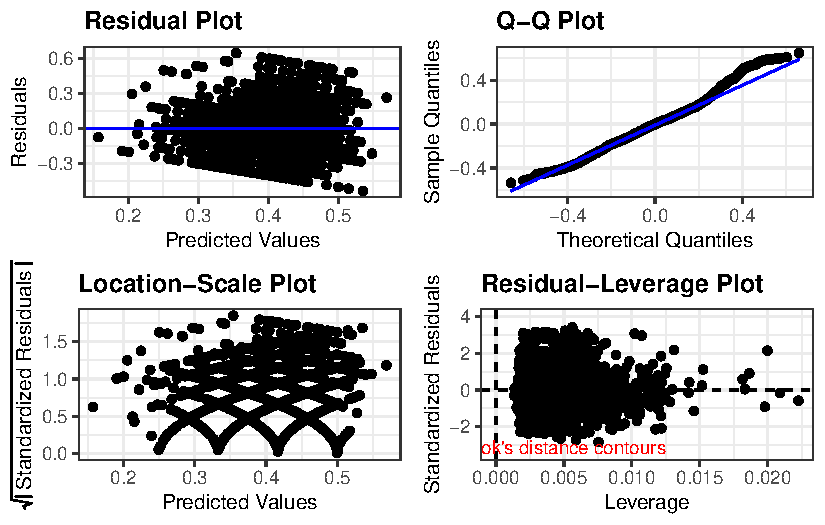
\includegraphics{Social-Isolation-in-China-jg-revised_files/figure-pdf/fig-resids-human-1.pdf}

}

\caption{\label{fig-resids-human}Human Interaction Model Residuals}

\end{figure}

\begin{figure}

{\centering 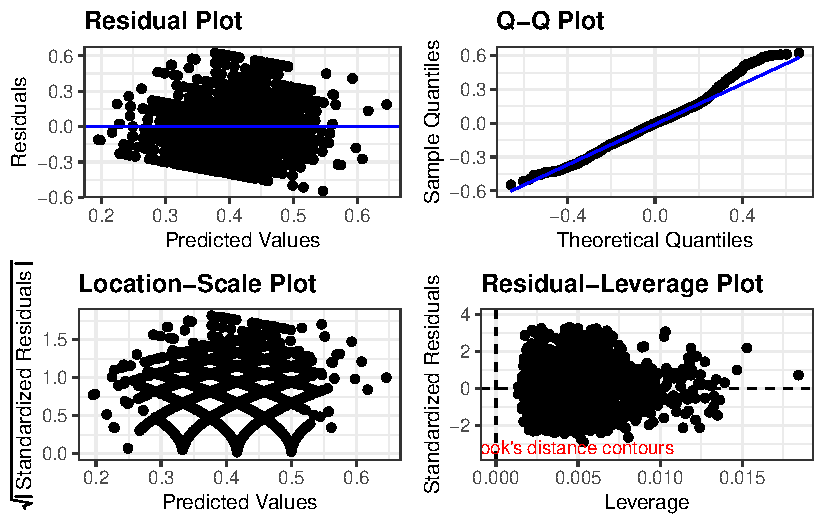
\includegraphics{Social-Isolation-in-China-jg-revised_files/figure-pdf/fig-resids-online-offline-1.pdf}

}

\caption{\label{fig-resids-online-offline}Online/Offline Model
Residuals}

\end{figure}



\end{document}
